\chapter{Applications}
\label{chap:applications}

In this chapter, we describe a few of the applications we have built using
Syndicate and Gaia.  In all cases, we show that the ability to construct
application-specific data flows allows us to tackle difficult data management
techniques in ways that both preserve backwards-compatibility with existing
applications, and preserve forward-compatibility with future storage features.
We show that applications do not need to be modified to leverage
new commodity services, and we show that data flows and gateway placement let us
solve data management problems in one logical place across all applications.

\section{Serverless Groupware}

% Groupware with Gaia
Groupware is a common Web application employed by users in the same
organization.  Groupware includes things like shared to-do lists, calendars,
shared documents, contact lists, and so on.

The data storage story for groupware today involves users being able to see a
consistent view of all of the users' groupware state, regardless of which
of their devices read or write it.  Since groupware is often used in sensitive
settings such as corporations, users have an expectation of privacy---by
default, their state is only visible to their devices.  Users must
\emph{explicitly} share data with other users (or the public).

In conventional groupware software, this is achieved by running a shared server.
The users in the same organization have read and write access to the server's
state, and the server resolves conflicts between writes and enforces access
controls.  In addition, the server takes advantage of its global view of the
users' state to build up derived state like edit histories and
backups.

We have used Gaia to design a groupware software library that can do all of these tasks,
but without requiring users to operate a globally-trusted always-on server of
their own.  Instead, they rely on external commodity cloud storage to host
encrypted application state, and use gateways running on their devices to
present a coherent read/write view of the users' data and incrementally build up
the same derived state.  This removes a single point of failure and a single
point of trust from groupware software, while also simplifying its design.

\subsection{Motivation}

Groupware software falls into two categories:  in-house groupware servers that
the users of an organization must maintain themselves, or out-sources groupware
servers that run in 3rd party servers.  There are undesirable 
trade-offs for both types of groupware.  In the first case, users incur an
ongoing operational cost for keeping the software up-to-date and keeping the
server running.  The advantage, however, is that they unilaterally control all
aspects of the server's data storage---including how often it gets backed up,
who can view the data, what kinds of derived state it makes, what version(s) of
the software it runs, and so on.

The second type of groupware is increasingly popular.  Companies like Microsoft
and Google each have suites of software-as-a-service offerings that take the
operational responsibilities out of the user's hands.  The advantage is that the
SaaS offerrings have potentially higher uptime and are managed by experts, and
are available at a predictable cost to users no matter how easy or hard it is to
maintain it.  The downside, however, is that the SaaS provider has global
visibility into the users' data, regardless of the users' desired privacy
settings.  If the SaaS provider is hacked, their groupware data can be exposed
to the public.  If the SaaS provider goes out of business, the groupware data
can be lost forever.

\subsection{The Role of SDS}

With Gaia, we can have the best of both worlds.  Users get all of the
operational convenience of SaaS with the privacy and data controls of having
their own servers.  Importantly, Gaia allows users to select whichever storage
providers they want without affecting the design of the groupware software. 
In addition, we show how ancilliary functionality like search indexing can be
implemented in Gaia gateways and reused in other applications (specifically,
shared between this application and our end-to-end encrypted email application).

The users rely in Gaia's SSI system to bootstrap data confidentiality and
authenticity.  The gateways in Gaia ensure that all data is signed and encrypted
when it leaves the device, such that only the user's designated recipients (if
any) can view it.  In addition, the groupware software uses Gaia to ensure that
applications are isolated from one another at the volume level---an application
client can only access application-specific state.

A key operational concern of groupware systems is that they must only allow
users in the same organization to view one another's data.  We use Gaia's
gateways to allow users to implement organization-specific checks when sharing
data to new users.  Specifically, the organization may require that users prove
ownership of a certain number and type of social media account, such as a
Facebook page or a Twitter feed, in order to receive read access.  These
social verifications are implemented at the SDS level, so all groupware
applications will be subject to a uniform set of access controls.

\subsection{Design}

Our groupware software is designed to run within the Web browser.  The
application logic runs as a Web page, and loads and stores the user's
credentials and data via a colocated Gaia node.  This allows us to decouple the
user experience and application functionality from the user group's shared
storage concerns.  For example, one user can store their data on Dropbox and
another user can store theirs on Google Drive, but the application can access
each user's data regardless via the Gaia node.  A system overview can be found
in Figure~\ref{fig:chap4-gaia-groupware}.

\begin{figure}[h]
   \caption{Design of serverless groupware with the Gaia SDS system.  Alice
   lists signed certificate graphs in her SSI user account data, as well as the
   list of her personal devices' public keys and social proofs.  While Alice can
   write to her storage from her private Gaia nodes, she can make her data
   available via a public Gaia node as long as her SSI account contains enough
   ``social proofs'' that she is a valid application user (and not a bot).  Bob
   uses this public gateway to discover and read her shared data.}
   \centering
   \includegraphics[width=0.9\textwidth,page=23]{figures/dissertation-figures}
   \label{fig:chap4-gaia-groupware}
\end{figure}

\subsubsection{Setup}

A user receives a volume for each groupware application she uses.  When she signs up for a specific
application, the groupware software inserts an application-specific set of keys
into the user's SSI account information, indexed under the application's name.  To provide
confidentiality, the user has the option of encrypting this routing information
such that only her trusted peers can discover that she uses it.  Her other
devices and other users' devices inspect her account in the SSI system to determine
which keys to use to authenticate the data she writes, as well as discover how
to access her storage (i.e. which Gaia nodes to contact, which storage providers
to contact, etc.).

\subsubsection{Sign-in}

The groupware software employs device-specific keypairs to allow the user to
sign in via multiple devices.  When the user signs in for the first time, her
device creates a volume for her and registers \emph{all} of her devices as
volume owners.  Then, when the user signs in from a different device, she can
still read and write data to her existing volume and administrate it.

The software ensures that her devices are aware of each other via a
``delegation record'' in her SSI account.  The delegation record lists all of
the user's device IDs and their public keys.  This way, when the user creates a
new volume, the software automatically grants all devices the volume owner
privileges.  To the user, it appears that they simply began using the app from a
separate device, just as they would have had it been a conventional Web app.

If the user wants to add or remove a device, she must re-generate her delegation
record with the current set of device public keys.
To do this securely, the software requires a quorum of signatures from a trusted
subset of her devices.  A delegation record will only be considered valid if it
is accompanied by a sufficient number of signatures from this trusted device
set.  For example, a user might require a signature from two of three of her
devices in order to add a fourth device or remove the third, and in doing so
tolerate the loss of one of her three devices.  This way, the user can control
which devices are allowed to write to her data while tolerating the loss or
compromise of a pre-configured set of them.

Both the quorum threshold and the public keys of the
trusted devices are listed in the user's SSI zone file.  Since changing the zone
file requires a blockchain transaction in the SSI system, there will be a
widely-replicated auditable log of each user's device key rotations.  This makes it
easy for users (and their employers) to check key lifetimes, and makes it
risky for attackers to attempt to change keys (since they cannot do so
silently).

When the user creates a gateway as part of signing in, her device will sign the
new certificate graph for the app's volume and make it available in her SSI account.  The
software authenticates data from the user by (1) looking up the user's ID in the
SSI system, (2) extracting the trusted device public keys and quorum threshold
from the zone file, (3) validating the delegation record, and (4) validating the
certificate graph against the delegation record.  The software caches
monotonically-increasing version numbers for the certificate graphs locally to
prevent stale certificate graphs from being reused.

\subsubsection{Reading and Writing Data}

Since a user gives each application its own volume, a groupware application like
a shared calendar spans the set of users' volumes.  Gaia ensures that when the
application client is loaded, it by default only has visibility into the
application-specific volumes the users have created (i.e. so a malicious
or buggy application cannot read another application's state).

The groupware storage interface addresses data by its key and owner user.  For
example, to read Bob's file \textit{today.cal}, Alice's application client would call
\texttt{get(``today.cal'', ``bob.id'')}, where \textit{bob.id} is Bob's username
in the underlying SSI system.  The sign-in process in Gaia
ensures that Alice's calendar application only discovers the routing information 
to Bob's calendar volume.

\noindent{\textbf{Read Authorization}}
When writing data, the user must ensure that it is readable by the same
organization members.  How does the user identify their organization members,
and how can the software ensure that only their organization members can read
their data?  We address the first by requiring each user to post a signed
proof-of-ownership within an existing social media account.  This gives a new
user a way to quickly judge whether or not someone's online personas belong to
the same person.

The user is free to choose which proofs are required for their
application, depending on the application.  For example, a cryptocurrency
investment application could require user to present signed KYC attestations
from the government and the user's bank that prove that the user is an
accredited investor.

Once a Gaia gateway knows which social media proofs are required by the
application, it will only accept read and write requests from users who have
made the requisite proofs.  To facilitate this check, users insert URLs to the
proofs within their SSI account linked to their names in the SSI system.

\noindent{\textbf{Searching}}
When writing data, the groupware software ensures that the local device's Push
stage indexes the contents of the file before encrypting and replicating it.
The Push stage also encrypts the index data with the viewers' public keys, so
the viewers will be able to search for the file by keyword.

The index itself simply links search terms to file names, as well as the number
of times the term shows up.  The index data is structured as a per-user prefix tree, so
that a search query only needs to fetch a narrow subset of the index to find
files with the search term.

Because the index is built up incrementally on
write by a client-side process, there is no need for a central server to
maintain global visibility into all the users' data.  This system instead
ensures that if Alice has made a file visible to Bob, then Bob will be able to
search Alice's index to find it.  Since groupware applications are meant to be
used by a known set of users, it handles search queries for a specific term by
quering each user's search indexes in parallel.

\subsection{Implementation}

Our groupware library is simply a Javascript library that facilitates user
sign-ins and application-specific volume creation and discovery.

% TODO: search indexing isn't implemented
% TODO; get line count on social proofs (look at gaia hub)

A to-do application, a media player, and a blogging application have been
implemented with our middleware.  The to-do application is only XXX lines of
Javascript, the media player has XXX lines, and the blogging application has XXX
lines.  All three of them use Gaia for storing their state.

\subsection{Discussion}

The power of SDS is apparent in its ability to meet the user's storage behaviors
independently of the applications.  Each user can keep their groupware data on
the storage providers of their choice, and in doing so, control their
availability and durability independently of one another and independently of
the applications.  At the same time, application developers do not need to care
about hosting user data, and do not need to worry about coupling their data to
specific storage systems.  In this example application, we additionally showed
how application-specific mutate flows can be used to implement complex
end-to-end behaviors (i.e. automatic content indexing and social proof checks to
control data access) without forcing each
application developer to implement similar functionality within their
code.  This makes individual applications simple to design and implement
while making strong, consistent guarantees to users about how their data will be
handled.

The main difficulty with giving users direct control over their groupware data
today is that it forced them to run a shared groupware server.  By instead
implementing what used to be server-side functionality as aggregation driver
stages, we were able to remove the need for a shared server while preserving the
user's control over their data.

\section{End-to-End Encrypted Email}

The ability for SDS systems to instantiate application-specific data flows gives
users the power to enforce data transmission and storage concerns in existing
protocols as well.  We demonstrate this by using Syndicate to construct
end-to-end encrypted email that addresses long-standing
usability concerns that impede the widespread use of PGP.

\subsection{Motivation}

Encrypted email is not a new concept.  However, it has proven notoriously difficult to
deploy~\cite{why-jonny-cant-encrypt}~\cite{why-jonny-still-cant-encrypt}
~\cite{why-jonny-still-still-cant-encrypt} due to the need for users to manage
private keys.  In addition, deploying end-to-end encrypted email over legacy
SMTP servers and clients leaves users vulnerable to two security flaws:  users
can only achieve end-to-end encryption if they all share keys, and users can
accidentally leak other users' cleartext when including new users in an email
thread.

\subsubsection{Using Private Keys}

Even if users did understand public key cryptography, they must still contend
with key distribution and key revocation.  Key distribution is not addressed by
the encrypted email systems studied.  However, existing methods---key escrows,
certificate authorities (e.g. S/MIME~\cite{smime}, DANE~\cite{dane},
x.509~\cite{x509}), and webs-of-trust are difficult to use securely, and easy to
use incorrectly.

Key escrows and certificate authorities are ``centralized''
entities that often live outside of a users' organizations, which makes it
difficult for users to reason about their trustworthiness.  Moreover, a
compromise of a widely-used certificate authority can lead to widespread
data exposure, which users may not discover until after harm has been done to
them (such as identity theft).

Webs of trust allow users to place their points of shared trust within
their organizations, but have a high operational cost to maintaining them.  This
is because trust is \emph{not} transitive by nature---if Alice trusts Bob and Bob
trusts Charlie, it does not follow that Alice trusts Charlie.  Users need to be
wary of the degree to which to trust their peers, and wary of the trust
judgements their peers will make.  Moreover, they must curate their webs of
trust to account for changes in the organization.  For example, if Bob is fired,
then all of Bob's coworkers must update their webs of trust to stop trusting his
emails.

Key revocation adds another layer of complexity.  Key revocation certificates
and signed key expiration dates do not go far enough in making encrypted email
usable.  If a user loses both their private key and their key revocation
certificate, then they have to get other users to re-establish trust in them
from scratch.  If the user's private key is compromised, then the attacker can
do arbitrary amounts of damage before the user can transmit their key revocation
certificate.  If the user loses their revocation certificate, or if the attacker
can stop the certificate from reaching the victims, then the user suffers the
full effects of the attack.

\subsubsection{Contacting other Users}

Even if users could reliably distribute and revoke public keys, conventional
email clients still allow users to communicate with others in insecure ways.
Users can bring harm to themselves by accidentally sending email in the clear
when they meant to encrypt it.  Also, users can bring harm to others
by accidentally divulging their communications by carbon copying
their cleartext in an email to a user who does not use encryption.

Neither existing SMTP clients (including Web clients) nor
SMTP servers address these problems.  SMTP clients do not help users with key
distribution or revocation, and they do not help the user discover whether or
not they have the right key.  Web SMTP clients are even less secure, because the
Web client offloads transmission to a remote server (which now must be trusted
by the user).  If the user wants to use another device to send an email, such as
a public terminal, they have to divulge their private key to the device.

SMTP is already ill-suited for encrypted communications because at a minimum the email's
sender and recipient must be readable by all SMTP servers between the sender and
recipients.  Also, due to its store-and-forward architecture, any messages
accidentally sent in the clear will be stored by the servers for a potentially
long amount of time.  Users do not get to choose which servers store and forward
messages, and users cannot ``unsend'' messages if they discover that they sent
them to the wrong recipient.

\subsection{The Role of SDS}

We have used Syndicate to build a email system that is backwards compatible
with SMTP, but automatically encrypts data end-to-end and ensures that users
discover each other's \emph{current} public keys automatically by way of its SSI
system.  Using our prototype, users can do the following:

\begin{itemize}
\item \textbf{Automate key management}.  Users do not need to interact with keys
at all.  Users do not need to trust external key escrows or certificate
authorities, and they do not need to participate in webs of trust.  Instead,
users rely on Syndicate's blockchain-powered SSI system to discover each other's
current public keys.

\item \textbf{Control where emails are hosted and who can request them}.
A user's message contents will
not be relayed through the SMTP network, but will instead be hosted in one or
more storage hosts of the user's choosing.  Recipients will instead download and
decrypt the message once they have discovered where it is hosted and have
obtained sufficient permission.

\item \textbf{Support sending to legacy users}.  Our system does \emph{not}
require both sender and recipient to use our client in order to achieve
better security than email.  If the recipient does not use our system, the sender has
the ability to contact the receiver while
preserving certain sender-chosen security properties.  For example, 
the sender can automatically share the message body via a private shared cloud storage folder
that only the sender and receiver can access, and send the sign-in URL via SMTP.

\item \textbf{Safely use untrusted devices}.  We use Syndicate's SSI system to
allow users to derive short-lived throw-away keys for signing and encrypting
messages on untrusted devices, like public terminals.  We show how to safely and automatically
distribute these keys.
\end{itemize}

\subsection{Design}

Our system follows a similar design to the Internet Mail
2000~\cite{internet-mail-2000}
proposal.  Users store their encrypted emails in a Syndicate volume, which they
use to selectively give recipients access to their messages.  The system uses
the SMTP network to allow senders to inform receivers when they have new
messages waiting for them (Figure~\ref{fig:chap4-syndicate-mail}).

\begin{figure}[h]
   \caption{Design of end-to-end encrypted email with Syndicate SDS.  Alice can
   send email from both a personal device and a public terminal; the latter of
   which gets assigned a temporary session key that expires shortly after being
   created.  Bob's client detects new mail from Alice via the legacy SMTP
   network by receiving a signed list of URLs that point to Alice's chosen
   storage services.  If Alice emails non-users of this system, her UG employs a
   custom ``message gateway'' (MG) type to Push the message payload to them
   while enforcing her custom security policies (such as ``store this message in
   a private shared Dropbox folder that the recipients can access and email them
   the URL'').}
   \centering
   \includegraphics[width=0.9\textwidth,page=24]{figures/dissertation-figures}
   \label{fig:chap4-syndicate-mail}
\end{figure}

\subsubsection{Setup}

Each user stores their preferred email address in the SSI system.
Alice sends a message to Bob by looking up Bob's account
information in the SSI system, and then obtaining his email address.

The system is designed to accomodate multiple devices owned by the user.  Each
device has its own Syndicate user account, which is used to create
device-specific gateways.  The user has an admin account, which she controls
from a trusted device and uses to add other devices (including pre-allocating
accounts for other devices).

When a user signs up for the system for the first time, she downloads and
installs a mailer daemon
that implements an SMTP and IMAP endpoint locally.  The user points their preferred email
client to the local mailer daemon to send and receive messages.  In addition,
the daemon implements an HTTP interface for serving the mail client encrypted
messages from the Syndicate volume.

The mailer daemon prompts the user to generate a device-specific
Syndicate user account and two gateways (a UG and an RG)
when it is installed.  The user does so by using her
admin account.  The installer wizard gives the user the option of pre-allocating
keys for user accounts and their gateways, which can be fetched and installed on untrusted devices
on-the-fly without requiring her to use her admin account again.  Their
keypairs are encrypted with a password of the user's choice, and stored to the user's
volume.

\subsubsection{Signing In}

Each device the user sends mail from receives its own keypair.  Each
device-specific key is associated with an optional expiry timestamp and
revocation certificate, which are stored in the user's Syndicate volume for
safekeeping.

Signing in with a new device requires ensuring that the device-specific private key is
available.  For devices the users trust, this is achieved simply by (1)
installing the software, and (2) allowing the device to register its public key
with the user's account in the SSI system.  An untrusted device, such as a
public kiosk, would receive a key with an expiry date and revocation certificate.
When the user signs out of the device, she would ``activate'' the revocation
certificate by moving it to a canonical path in her volume.  The timestamp
ensures that the key expires nonetheless if the user is unable to successfully
sign out.

The device-specific key state includes the device-specific user account and the
device-specific gateway keys that the mailer daemon will use to interact with
the volume.  Each devices' gateways only write to one directory of the volume,
and mark their files as read-only by other devices (which the MS enforces).
The mailer daemon develops a coherent view of the mailboxes by listing all of
the devices' directory states.

In addition to creating device-specific Syndicate keys, the software also
creates a generic read-only UG and read-only RG whose private keys are publicly readable
and exposed in the volume.  These gateways are meant to allow recipients to access
the volume's ciphertext, so the designated recipient can decrypt them.
They are configured in the certificate graph to only have read capabilities, and
to only serve on \texttt{localhost}.  This ensures that all of the user's other
gateways will ignore them, and that anyone can run them on their computers to
access the inbox data.

\subsubsection{Sending and Receiving Mail}

The mailer daemon implements a Syndicate UG and RG (e.g. as subprocesses).
The UG implements the SMTP
and HTTP endpoints, and the RG uploads messages to the user's preferred storage
service (such as their personal Dropbox folder, or an S3 bucket).

When the UG receives an outgoing message, its \texttt{serialize()} driver method inspects the
message for the recipient, and automatically looks up the public key in the SSI
system to encrypt the message to the recipient before sending it to the RG.
\emph{This way, the sender is never involved with selecting the key for a
recipient user.}  The software additionally makes a copy of the sent message encrypted with the
sender's public key, and stores it into the device's ``sent'' mailbox.

The mailer daemon informs the recipient that they have a message waiting for
them by sending a small amount of control-plane information to the recipient's
email address via SMTP.  The control-plane information is signed by the sender,
to prove its authenticity to the recipient.  It identifies the path to the
message in the volume, as well as the hash of the ciphertext.

The recipient's mailer daemon polls the user's inbox for these specially-crafted
messages.  Upon discovery, it fetches, authenticates, and decrypts the message,
and locally stores it so the user's local mail client can read it as a normal
email.  It does so automatically as part of the \texttt{deserialize()} driver
method in the UG---the method only succeeds if the message could be
authenticated.  The control plane SMTP message's sender email address
is used to look up the user's device keys in the SSI system to perform the authentication.
\emph{This way, the receiver never needs to select the key for the
sender to authenticate the message.}.

Once the recipient daemon has fetched the cleartext, it encrypts and backs up a
copy via its RG for safe-keeping (i.e. in case the sender deletes their volume).
This allows the sender to garbage-collect sent emails at a later date.

If the sender includes multiple recipients, or includes a new recipient part-way
through the email chain, their mailer daemon is able to detect this and ensure
that the previous conversation is kept secret.  This is achieved by having the
local RG in the mailer daemon remember which email threads have which recipients,
and ensure that their respective messages are re-encrypted before transmission.
The user would need to explicitly copy and share any parts of the previous
conversation threads in order to expose them to the new recipient.

\subsubsection{Legacy Compatibility}

It is important to recognize that when it comes to email, the correct way to
send a message depends on the recipient, the content, and the context in which
it is sent.  Two friends exchanging vacation photos do not need the same
security guarantees as an anonymous informant communicating with a law
enforcement agent.

One of the major drawbacks of PGP is that cannot work if either the
sender or recipient do not use it.  This significantly limits the set of senders
and recipients.  Moreover, PGP-encrypted messages are easy to spot in SMTP
traffic, which makes it easy for network eavesdroppers to identify users who
have something to hide.

What is needed is for senders and receivers to be able to communicate even if
one of them does not use PGP-like encryption.  The approach we have taken is to
make it easy for the sender to control how the message will be delivered, while
allowing messages to be discovered by the recipient over legacy SMTP.  The
sender is free to set up the delivery process to implement the security
guarantees as fit, subject to what she knows about the recipient and subject to
the contents of the message.  For example:

\begin{itemize}
\item The sender can encrypt the message with a password known to the recipient,
and send the message body in a common document format, like Microsoft Word or
PDF, that the recipient can open and decrypt with already-installed software.
This provides the confidentiality of PGP.
\item The sender can replicate the message to a shared private storage provider
like a Dropbox folder or \texttt{git} repository, and send the
recipient the URL over SMTP.  The replication by the sender and the access by
the receiver can be performed over HTTPS.  While this does not provide the same
degree of confidentiality and authenticity as PGP, it guarantees that as long as
the certificate authorities are trusted, only the sender, the recipient, and the
storage provider can view the message (but the SMTP servers cannot).
\item The sender can select which network the host will use to use to transmit the data, based on
the recipient.  For example, an enterprise user could require all messages sent
to the company SMTP server to be sent only through their computer's
VPN interface.  This ensures that all email messages sent by employees are
visible only to the company and the recipient.
\end{itemize}

These examples do not provide the same strong guarantees of PGP, but they are
better than relying only on legacy SMTP for email.  While they can all be done
today in an ad-hoc manner, Syndicate lets us ensure that they are all executed
automatically and consistently.  Moreover, the way we implement these features
allows them to be reused in multiple different contexts, giving senders the
ability to \emph{compose} different features to create a custom message
transmission process.

Addressing legacy compatibility is a practical application of Syndicate's custom
gateway types.  We have the RG's
Push driver stage (1) reassemble the Pushed chunks received from the UG
(embedded in the email client) back into the original email, (2)
scan the certificate graph for gateways with a type identifier specific to the
email client, and (3) forward the reassembled email to them for further
processing.

When the email-type gateway receives the message, it inspects the message
headers and runs a user-specified program based on the recipient address.  The
user-specified program is responsible for actually transmitting the email.
For example, each of the above examples can be implemented with separate
programs.

The programs themselves are part of the email-type gateway's driver.  The user
deploys them to her volume by updating the certificate graph.  Since the volume
spans all of her devices, each of her devices will have the most up-to-date
transmission policies activated whenever the user sends a message.

\subsubsection{Search Indexing}

Since all messages are encrypted client-side, there is no option for server-side
message indexing.  Instead, the user's RGs incrementally build up a
word-to-email index as part of their Push stage logic, just as they do in the
serverless groupware example.  The index itself is
encrypted with the user's public keys, so it is visible only on the user's devices. 
In fact, the code to maintain the users' indexes can simply be re-used by the
RGs without affecting the design or implementation of the mail clients.

There are two reasons we offload search indexing to the RGs instead of allowing
applications to handle this.  First, this lets us preserve the index across all devices. 
This is especially important for Web clients, which cannot easily store a large amount of state
locally (HTML \texttt{localStorage} is limited to 5MB, for example).  Second, it
makes it easier to implement additional features like spam filtering, described below.

\subsubsection{Spam Filtering}

One difficulty with encrypted email today is that the servers cannot filter spam,
since they cannot read the messages.  We address this in four ways.

First, we have the RGs in a user's volume build
up a \emph{shared} set of classification data from user input.  When the user
moves data to the ``spam'' mailbox, the RG driver's Push stage generates and
a feature vector from the cleartext and stores it in a shared storage
provider.  This allows
users to share each others' spam feature information.

The shared storage itself is implemented as a separate, 3rd party volume that enforces write-once read-many
access patterns, and tracks which users add which features.  That is, the RGs to the volume do not allow a record to be
written more than once, and do not allow records to be deleted (except by the
volume owner).  This ensures
that users do not accidentally clobber one another's writes, and a malicious
user (such as a spammer) cannot erase the feature vectors.  If it is later
discovered that a particular user's records were written with malicious intent,
they can be later removed by the volume owner.

This arrangement is similar to existing 3rd party spam detectors such as
Spamhaus~\cite{spamhaus}, where a 3rd party aggregates spam information 
on behalf of many users.  The spam volume owner would aggregate the spam
information to train a spam classifier, and write the classifier parameters
to the volume.  A user's mailer daemon would connect to the volume in a read-only fashion
to read the classifier parameters, and use them to classify the user's inbound
messages as spam or not spam.  Because the volume is shared across many users
(and can be replicated by any user), the users are able to avoid spam-detection
service lock-in because they can (1) independently calculate the spam classifier
parameters, and (2) come up with their own, better classification system if the
spam volume owner does not do a good enough job.

Our second anti-spam feature is that by design, the user pays for storing messages to recipients.  Since each
recipient has a different public key, the user must encrypt a message for each
recipient.  Since the user may not want users to know that others have received
the same message (i.e. to implement blind carbon copy semantics), the user must
ensure that each user receives a different ciphertext.  As a result, a spammer
must store a lot of state to spam many users at their own expense.  This
disincentivizes, but does not completely remove, bulk spam.  This is similar to
the Internet 2000~\cite{internet2000} webmail proposal.

Our third measure is to take advantage of the fact that the SSI system is implemented on top of
a public blockchain.  This feature allows for some interesting anti-spam mechanisms.  A recipient can require the sender
to include a ``proof-of-payment'' on the message, generated by a transaction on the
underlying blockchain.  This would have the effect of both rate-limiting
spammers and making emailing users prohibitively expensive to do at scale.  It
would also allow senders to prioritize messages by paying higher fees This
is a technique employed by 21.co~\cite{21co-messaging}, for example, whereby a user will only see a
message if the sender has paid a minimum amount of money required by the
recipient.

Our fourth measure is to re-use a concept from our Gaia groupware to require
that a sender provide sufficient proofs in the SSI system that they are a
legitimate human being, and not a bot.  For example, a recipient can enforce a
default anti-spam policy whereby a sender must supply evidence in their SSI
account that they own at least five unique social media accounts, and that the
accounts undergo a minimum amount of activity.  This makes it hard to send
spam at scale because (1) the spammer would need to circumvent all of the social
media systems' ant-bot mitigations, and (2) if the spammer gets caught, they
have to register a new identity in the SSI system (necessitating a blockchain
transaction).  Since the blockchain itself grows at a fixed rate, and since
blockchain peers effectively bid on the ability to write new transactions, a
spammer could not easily register many identities without paying a high price
(i.e. the price gets higher the faster the spammer tries to register new
identities).  This allows us to overcome the limits of prior proof-of-work
techniques~\cite{anti-spam-proof-of-work} which either had a fixed proof-of-work
threshold or a threathold that increased independently of the system's usage.

All four of these techniques would be implemented by the Acquire stage of the
mailer daemon's RG.  This ensures that all email clients automatically benefit
from these mechanisms without modification.

\subsection{Implementation}

Our prototype system, SyndicateMail, is implemented in 4100 lines of Python and
1700 lines of Java.  It implements end-to-end encryption across multiple devices
and offers legacy compatibility with SMTP.

We were able to re-use the search indexing
logic from Gaia to implement search indexing in Syndicate.  We simply had the RG
driver run the indexing logic as a subprocess in a \texttt{node.js} VM.  The
spam filtering is carried out simply by passing the text through an existing
spam-detecting system such as \texttt{spamd}~\cite{spamd} or \texttt{spam-assassin}
~\cite{spam-assassin}, and only forwarding the email text if it is not spam.
These both demonstrate the power of Syndicate's gateway model---we 
derived complex domain-specific data-processing logic by composing
already-written but unrelated programs in a pipeline-like fashion.

\subsection{Discussion}

In terms of the number of patches to write, it would be costly to implement this email system without
SDS.  Each email client would need to be patched to store its state to the
storage provider of the user's choice, whereas the use of Syndicate ensures that
we only need to port storage serivces once.  By moving data signing,
encryption, decryption, and verification to the storage layer, and automating
them by using Syndicate's SSI system to bootstrap key trust, we were able to
make existing email clients compatible with encrypted email without forcing
users to understand public-key cryptography.  By using gateways to represent the
capabilities of each device, we were able to preserve the convenience users expect from Webmail
without forcing them to manually copy private keys between devices.

Filtering spam and preventing accidental cleartext disclosure are problems
that require the system to inspect email contents on the user's behalf.  We
achieved this by having the user's RGs carry out this inspection locally,
instead of foring the user to trust an external SMTP server to do so on their
behalf.  This was crucial to ensuring end-to-end message confidentiality, and
was required to be implemented at a layer \emph{beneath} email clients to ensure
that the user's choice of client did not alter the system's ability to ensure
message confidentiality and prevent spam delivery.  We were able
to address both of these problems by
allowing the user to run application-specific aggregation driver
stages interposed between their personal devices and the rest of the network.

\section{CDN-accelerated Scientific Data Staging}

Scientific computing is increasingly an inter-organizational effort.  Data is
generated and stored in the labs where a scientific instrument or dataset is
curated, and then shared across the world with collaborators.  Similarly,
collaborator labs publish their data analyses, which get pulled by other labs
(and classrooms) for further consumption.

We have used Syndicate to implement a cross-site data processing framework that
allows scientists to take advantage of commodity cloud storage and CDNs to host
and deliver data to each lab.  For dataset curators, we have reduced the task of
exposing a dataset to collaborators to running a Syndicate AG that can crawl the
dataset (with a dataset-specific driver) and serve chunks of it to downstream
UGs.  For dataset readers, we have reduced the task of accessing a dataset to
fetching a dataset-specific Docker~\cite{docker} image that mounts the dataset
as a read/write filesystem backed by the dataset AG, an intermediate CDN, and
the user's personal cloud storage.

\subsection{Motivation}

The main motivation for considering an SDS approach to scientific data storage is
that due to the nature of the data they gather, each lab will have its own data curation
policies, its own unique data access patterns, and its own policies on when to
share data and in what format it will be available.  There is not a
one-size-fits-all approach for hosting scientific data, and labs will need to tailor
their storage systems to meet their specific needs (especially since their needs
change over time, depending on the nature of the data they produce).

This need to accomodate changing data storage and access policies is evident in
the evolution and wide success of state-of-the-art scientific storage systems
like iRODS~\cite{irods}, which offer
user-programmable policies (``rules'' and ``microservices'') that allow
individual scientists, project teams, and entire labs to programmatically
specify their curation policies and have them automatically enforced.
Indeed, we consider iRODS to be an SDS system.

We want to use commodity CDNs and cloud storage to help iRODS deployments
handle ``fan-out'' data distribution cases, where many labs across the wide
area want to read existing datasets and write back changes that will be
incorporated into the iRODS dataset.  CDNs would let individual iRODS
deployments scale up the number of reads they could service.  Commodity cloud
storage would allow users to host the results of their computations and share
them with their lab mates and peers before generating and preserving a
``curated copy'' of the data back to iRODS.

\subsection{Challenges}

Augmenting existing systems like iRODS
with commodity infrastructure introduces challenges of
its own.  We cannot simply place a CDN in between iRODS and remote readers for
three reasons:

\begin{itemize}
\item \textbf{Protocol Incompatibility}.  CDNs are designed for Web content
acceleration, which implies caching ``small'' files and
using HTTP as the data delivery protocol.  However,
iRODS does not speak HTTP.  A protocol translation layer will be required.
\item \textbf{Cache Unfriendliness}.  CDNs are designed for caching lots of
``small'' files---i.e. website assets like HTML or CSS that are not usually
gigabytes in size.  However, iRODS data can be extremely large, and clients may
only even want a small range of an iRODS file.  Serving iRODS data with a CDN
while getting good bandwidth will require file-level fragmentation and reassembly
on both the producer's and consumers' endpoints.
\item \textbf{Concurrent Writes and Reads}.  iRODS is a read/write datastore.
While some users are reading from a file, another user can be writing to it.
Avoiding this today requires \emph{manual coordination} between readers and
writers.  A writer needs to mark a newly-written dataset as read-only, and a
reader needs to manually download and stage a replica on the compute cluster to
ensure that subsequent writes do not result in corruption.  This is a tedius
process for writers, and time-consuming and potentially wasteful for readers
(especially if the reader does not need the entire file).  However, removing both of
these pain points cannot be achieved simply by placing a CDN in between the
iRODS deployment and the wide-area readers, since the CDN can accidentally serve
stale data fragments (i.e. the writer cannot invalidate cached CDN data).
\end{itemize}

In addition, sharing the results of local computations and generating a
dataset to write back to iRODS has its own challenges:

\begin{itemize}
\item \textbf{Replica discovery}.  Suppose a scientist reads some data from iRODS,
runs some local jobs on it, and saves its results to the lab's shared Dropbox
folder.  How do the scientist's peers find the data, so they can run their own
analysis on it?  A strawman solution is to simply email the links to the peers.
However, this introduces a manual, tedious process for sharing data.  Can we
automate data discovery with Syndicate?
\item \textbf{Replica write-back}.  Not all scientists who generate new data
have accounts on the iRODS system.  How do they get their results incorporated
into the iRODS copy?  More specifically, how do they discover the set of
authentication credentials?  How does the data ingress server authenticate the
user if they do not have an iRODS account?  A strawman solution here is to find
and email an iRODS user with sufficient privileges and ask them to incorporate
the changes.  But how do we do this automatically, without requiring more humans
in the loop?
\end{itemize}

We can address all of these with the right configuration of Syndicate gateways.

\subsection{The Role of SDS}

The need for software-defined storage in scientific computing is not new.  The
labs that gather and share scientific data must already do so according to
data-specific rules.  These include rules governing storage aspects like
national export controls, disclosure of proprietary or potentially dangerous information, and
even mundane concerns like ensuring the data appears in the correct format.

Prior to systems like iRODS, these rules had to be enforced either within the
scientific computing applications, or within a bespoke storage system.
Enforcing the same rules across many labs' applications poses a high cost of
coordination, since each lab's applications must be audited for compliance.
Enforcing a set of rules within a bespoke storage system requires constructing a
bespoke storage system for each rule set.  Allowing a storage system to have its
curation rules programmed at runtime without changing the application-facing
storage APIs is the ``sweet spot'' of SDS for scientific computing.

In this particular application, we extend an existing SDS system (iRODS) with
Syndicate to allow iRODS workflows to take advantage of commodity infrastructure
(CDNs and cloud storage) without affecting the application-facing storage APIs.
Crucially, we do so in a way that \emph{preserves} the data owner's existing iRODS
rules in a global setting, while allowing the owner to specify additional
rules within Syndicate to specifically control how data is disseminated once it
leaves iRODS.

\subsection{Design}

An iRODS system can store many different datasets, and each dataset can have its
own access control policies set by the owner.  These are enforced internally by
iRODS when other users attempt to access the data.

\begin{figure}[h]
   \caption{Overview of CDN-accelerated scientific data.  The iRODS deployment
   is private, and accessible only via the AG and RG (which run in trusted
   networks).  Remote UGs leverage the MS and CDN to read cached but fresh data,
   regardless of the CDN's caching policies.  When UGs write data, they do so
   via the trusted RG which sends the changes to the proper datasets.  All the
   while, the AG keeps the MS metadata consistent with writes from non-Syndicate
   iRODS clients by subscribing to a (iRODS-specific) message queue.}
   \centering
   \includegraphics[width=0.9\textwidth,page=25]{figures/dissertation-figures}
   \label{fig:chap4-syndicate-datasets}
\end{figure}

Our strategy for distributing each dataset to remote readers is to allow an
iRODS user to ``export'' their dataset by way of a Syndicate AG, and later
``import'' changes to it by way of an RG.  Both the AG and RG run with the
permissions of the dataset owner (Figure~\ref{fig:chap4-syndicate-datasets}).

The AG crawls the owner's dataset using
our iRODS driver and exports individual file metadata to the Syndicate MS.
It runs within a demilitarized zone (DMZ) on the network, linking the iRODS data
to the outside world.  It acts as an origin
server to the CDN and uses its iRDOS driver to load and serve file data as blocks and
manifests to downstream readers.  A dataset owner can run many AGs, and can have
different AGs index different parts of the dataset.

The RG accepts inbound write requests from external users who want to
incorporate their changes to the dataset owner's files.  It also runs in the
DMZ, so it can receive inbound requests.  It uses the dataset owner's
credentials to access iRODS.

The dataset owner's AG and RG operate in \emph{separate} volumes---one for
distributing data to readers (backed by the AG), and one for accepting new data
from writers (backed by the RG).  A remote user would mount one or both volumes
in order to get read-only or read/write access.

\subsubsection{Read Authorization}

Each AG acts as an origin server to one or more downstream CDNs.  It does not
have direct contact with UGs at the edge, which initiate access flows.  This is
acceptable for public datasets, where no read authentication is needed.

If read confidentiality is desired, the AG will encrypt its
manifests and blocks with the `serialize()` stage of its driver.  It uses each
UG's public key from the certificate graph to send it a shared secret.  The
encryption is deterministic, such that two requests for the same chunk will
resolve to the same ciphertext.  This allows multiple UGs to leverage the CDN
for read availability without the CDN being trusted with data
confidentiality---UGs reading the same chunk will fetch the same ciphertext, and
the CDN will only cache one copy of the chunk's ciphertext.

The two drawbacks of this configuration is that the CDN can still see access patterns
on the ciphertext, and anyone who can read from the CDN can fetch ciphertext.
This may allow unauthorized principals to infer information about the data being
accessed.  If scientists wish to avoid this outcome, then the solution is to use
a trusted CDN that will carry out authentication at the edge.

Regardless of the disposition of the CDN, the scientific applications are none
the wiser as to the authentication steps taken by the UG.  This is
because the UG's driver handles the interfacing with the CDN.  If the
UG needs a decryption key to read chunks (i.e. for read confidentiality), then
the volume owner can distribute them to the UGs by sharing it through the
certificate graph (encrypting the decryption key with each UG's public key).  If
the UG needs an access credential to the CDN (i.e. for metadata
confidentiality), then the volume owner can distribute them in the same manner
and write the CDN driver to have the UG submit it in the appropriate
CDN-specific manner.

\subsubsection{Write Authorization}

Each RG acts as an aggregation point for data generated by external UGs.
Unlike the read path, the UGs have direct contact with the RG on the write path.
As such, the UG's Push stage can ensure data confidentiality across the wide
area simply by contacting the RG via HTTPS.  The UG and RG configurations in the
certificate graph would be structured to include TLS certificates for each
gateway, so the RG could authenticate UGs and UGs could authenticate the RG.

Only the RG has write access to the iRODS deployment.  The volume owner installs its
iRODS credentials via the certificate graph as well (ensuring that they are
confidential and up-to-date by encrypting them with the RG's public key).

The RG has the ability to perform write authorizations on a per-file and even a
per-file-region basis.  This is because the UG informs the RG which file it
writes to (i.e. as part of the manifest and block information it Pushes), and it
informs the RG whenever it renames or truncates a file.  The RG has the ability
to NACK operations that do not conform to the volume owner's policies.  For
example, a UG may be denied a request to rename a file into a separate
\textit{\$HOME} directory in order to prevent users from gaining control of
parts of the dataset.

\subsubsection{Preserving Existing Policies}

From iRODS's perspective, the AG and RG are the only readers and writers to a
particular dataset.  Moreover, their reads and writes reflect the global
sequences of reads and writes initiated by wide-area users.  As such, the
volume owner retains the power to \emph{globally} enforce her iRODS-specific rules on data
accesses---any gateway-initiated accesses must also conform to the
already-deployed iRODS rules.

The volume owner can also set \emph{per-user} rules within her
gateways' drivers.  Importantly, iRODS does not need to be aware of the
Syndicate users, nor aware of the per-user policies that the gateways enforce,
since they occur in a separate layer.

As a result, scientists do not need to do any extra work or carry out any extra
configuration steps to begin sharing their iRODS-hosted data with off-site users.
All of their iRODS-local access policies continue to apply, and the scientist
has the \emph{option} of creating more-detailed rules within Syndicate.

\subsection{Implementation}

We have deployed a variant of the Akamai~\cite{akamai} CDN to
OpenCloud~\cite{opencloud}, a federated computing platform similar to PlanetLab.
The CDN is operated by the OpenCloud developers and is made available to all
participating sites.

We have deployed several AGs on top of the iRODS deployment at the University of
Arizona, and registered them as origin servers on the OpenCloud-hosted CDN.  In
addition, we have made several Docker images~\cite{syndicate-website} and a dataset-mounting
tool~\cite{sdm} available for the general public to try out the system.

When a user downloads and installs a read/write Docker image, she receives two
mounted volumes---the read-only volume containing the dataset, and a read/write
volume for writing the results of her experiment.  She and her collaborators
will see each other's results when they are written.  We run several RGs that
write back her and other users' results to iRODS, as well as to a temporary S3
bucket that gets cleared every 24 hours.

iRODS-compatible applications interface with iRODS through FUSE and through a
set of command-line utilities.  We have created a FUSE filesystem to preserve
compatibility, and we are working on a set of iRODS-compatible CLI tools.

In addition, we have implemented a Hadoop filesystem plugin that allows Hadoop
computing jobs to pull data from iRODS via Syndicate and the underlying CDN.
The HDFS plugin gives the job scheduler insight as to where Syndicate UGs have
locally cached chunks, so it can schedule tasks on nodes that already have the
data present.

Our iRODS-facing driver is ~1900 lines of Python, of which ~640 are specific to
iRODS, ~375 are specific to the AG, and ~375 are specific to the RG.  Our
UG-specific CDN interfacing driver is ~100 lines of Python.  Our Hadoop plugin
is ~2300 lines of Java.

\subsection{Discussion}

Again, the utility of using SDS to link existing scientific data stores to
commodity cloud infrastructure is visible in the fact that we are able to ``slap
on'' extra storage and data distribution capacity with little effort.  The
marginal cost of adding support for new storage and CDNs in terms of lines of
code is small enough that it can be achieved in as little time as a couple
hours, including testing.

The key benefit to iRODS users in particular is that the iRODS system needs no
special modification to be made compatible with the CDN.  This is because
SDS lets us port the CDN and storage to iRODS, instead of the other way around.
In doing so, iRODS-compatible applications (and even applications that only use
iRODS indirectly, such as Hadoop jobs) can transparently benefit from its extra
availability without having to overcome our aforementioned challenges.

\section{Remarks}

In these sample applications, using an SDS system to host data allows us to
tackle several difficult problems.  In all three examples, we see
that \emph{SDS provides semantic independence from storage systems} (i.e.
portability).  By both wrapping individual services behind well-defined service driver models, and by
allowing the volume owner to inject aggregation driver logic inbetween the
application endpoints and the underlying services, we were able to ensure that applications
had access to a persistent data store that behaved exactly they way they needed
\emph{as if the application was using a purpose-built storage system}.

In all cases, we realized the desired application-specific storage semantics by
implementing gateways to handle unrelated storage concerns, and composing them
together into handle access and mutate flows.
In our groupware example, users host their data on whatever storage providers they want
while deploying gateways to enforce arbitrary access controls and maintain globally-visible search
indexes.  In our email example, users host
their email in whatever storage providers they want and deploy gateways to
implement spam filtering, search indexes, message prioritization.  In our scientific
computing example, users augment existing storage systems with the CDNs and cloud
storage of their choice while deploying gateways to preserve the original system's global access
control rules and end-to-end consistency semantics.  Being able to compose
gateways was crucial to preserving storage semantics across organizations, since
in all cases there were sensitive operations like access controls and encryption
that could only be allowed to execute on certain computers.

The separation between aggregation drivers and service drivers proved useful in
practice.  Having these two layers of indirection allowed us to reuse service
drivers across different applications, and even across different SDS systems.
In doing so, \emph{SDS reduced the marginal cost of adding support for new
services to writing a single driver}.
Neither the aggregation driver logic nor the application need to be
patched when a new service becomes available.  Instead, a volume owner only
needs to deploy an updated service driver to her relevant gateways.

A slew of engineering problems were solved by
designing the storage layers of these applications to treat users as sovereign
from their organizations and as the true owners of their data.
For groupware, gateways authenticate and vet new users who would
share their groupware data.  For email, gateways discover the
sender and recipient public keys automatically and preserve end-to-end
authenticity and confidentiality.  For scientific data sharing,
gateways preserved dataset access controls regardless of the infrastructure used
to ship the data to external consumers.

Two of these applications---the scientific data sharing application and the
groupware application---have been successfully used in production settings.
There are many interested third parties who are in the process of developing
additional applications on top of Gaia~\cite{blockstack-app-fund}, and the NSF
and Internet2 have expressed interest in using Syndicate for cross-lab data
sharing~\cite{nsf-grant}~\cite{conversation-internet2}.
